\documentclass[20pt,a4paper]{report}
\usepackage[T2A,T1]{fontenc}
\usepackage[utf8]{inputenc}
\usepackage{blindtext}
\usepackage[russian]{babel}
\usepackage{mwe}
\usepackage{graphbox}
\usepackage[document]{ragged2e}
\usepackage[margin=50pt]{geometry}
\usepackage{longtable}
\usepackage{fontspec}
\usepackage{float}
\usepackage{titlesec}
\usepackage{setspace}
\usepackage{minted}

\usepackage{hyperref}
\hypersetup{
    colorlinks,
    citecolor=black,
    filecolor=black,
    linkcolor=black,
    urlcolor=black
}

\setstretch{1.5}
\graphicspath{{./images/}}
\setmainfont{LiberationSerif}
\setmonofont{Hack}
\titleformat{\chapter}{\normalfont\LARGE\bfseries}{\thechapter}{1em}{}
\titleclass{\chapter}{straight}
\titlespacing{\chapter}{0pt}{0pt}{5pt}[25pt]


\begin{document}
	\begin{titlepage}
		\begin{minipage}{0.3\textwidth}
		
\includegraphics[scale=0.03]{logo.png}	
		\end{minipage}
		\begin{minipage}{0.6\textwidth}\centering
			\textbf{
				Министерство науки и высшего образования Российской Федерации
				Федеральное государственное бюджетное образовательное 
				учреждение высшего образования
				«Московский государственный технический университет
				имени Н.Э. Баумана (национальный исследовательский университет)»
				(МГТУ им. Н.Э. Баумана)
			}	
		\end{minipage}
	
		\vspace{5cm}
		\centering
		\Large
		\textbf{
			Лабораторная работа №3 \\
			по курсу «Разработка интернет-приложений» \\
		}

		\vspace{6cm}
		\begin{flushright}
			Выполнил \\ 
			студент группы ИУ5-54Б \\ 
			Сысойкин Е.М. 
		\end{flushright}
		\vspace{5cm}
		Москва, 2020
	\end{titlepage}

	\chapter{Общее описание задания}
	\large
	\qquad Задание лабораторной работы состоит из решения нескольких задач. \\
	\qquad Файлы, содержащие решения отдельных задач, должны располагаться в пакете lab\_python\_fp. Решение каждой задачи должно раполагаться в отдельном файле. \\
	\qquad При запуске каждого файла выдаются тестовые результаты выполнения соответствующего задания. \\

	\chapter{Выполнение задания}
	\section{Задача 1(файл field.py)}
		\qquad Необходимо реализовать генератор field. Генератор field последовательно выдает значения ключей словаря. Пример: \\
		\small
		\begin{minted}{python}
goods = [
	{'title': 'Ковер', 'price': 2000, 'color': 'green'},
    {'title': 'Диван для отдыха', 'color': 'black'}
]
		\end{minted}

		\mintinline{python}{field(goods, 'title')} \large должен выдавать \'Ковер\', \'Диван для отдыха\' \\

		\small \mintinline{python}{field(goods, 'title', 'price')} \large должен выдавать \\ 
		\small \mintinline{python}{{'title': 'Ковер', 'price': 2000}, {'title': 'Диван для отдыха'}}
		\large
		\begin{itemize}
			\item В качестве первого аргумента генератор принимает список словарей, дальше через *args генератор принимает неограниченное количествово аргументов. 
			\item Если передан один аргумент, генератор последовательно выдает только значения полей, если значение поля равно None, то элемент пропускается.
			\item Если передано несколько аргументов, то последовательно выдаются словари, содержащие данные элементы. Если поле равно None, то оно пропускается. Если все поля содержат значения None, то пропускается элемент целиком.
		\end{itemize}

		\subsection{Код}
			\small
			\inputminted[tabsize=4, linenos]{python}{field.py}
			\large

		\section{Задача 2 (файл gen\_random.py)}
		\qquad Необходимо реализовать генератор gen\_random(количество, минимум, максимум), который последовательно выдает заданное количество случайных чисел в заданном диапазоне от минимума до максимума, включая границы диапазона. Пример: \\

		\small \mintinline{python}{gen_random(5, 1, 3)} \large должен выдать 5 случайных чисел в диапазоне от 1 до 3, например 2, 2, 3, 2, 1 \\
		
		\subsection{Код}
			\small
			\inputminted[tabsize=4, linenos]{python}{gen_random.py}
			\large

		\section{Задача 3 (файл unique.py)}
		\qquad Необходимо реализовать итератор Unique(данные), который принимает на вход массив или генератор и итерируется по элементам, пропуская дубликаты. \\

		\qquad Конструктор итератора также принимает на вход именованный bool-параметр ignore\_case, в зависимости от значения которого будут считаться одинаковыми строки в разном регистре. По умолчанию этот параметр равен False. \\

		\begin{itemize}
			\item При реализации необходимо использовать конструкцию **kwargs.
			\item Итератор должен поддерживать работу как со списками, так и с генераторами.
			\item Итератор не должен модифицировать возвращаемые значения.
		\end{itemize}

		\qquad Пример: \\
		\small \mintinline{python}{data = [1, 1, 1, 1, 1, 2, 2, 2, 2, 2]} \\ \large 
		Unique(data) будет последовательно возвращать только 1 и 2. \\

		\small \mintinline{python}{data = gen_random(1, 3, 10)} \\ \large
		Unique(data) будет последовательно возвращать только 1, 2 и 3. \\

		\small \mintinline{python}{data = [‘a’, ‘A’, ‘b’, ‘B’, ‘a’, ‘A’, ‘b’, ‘B’]} \\ \large
		Unique(data) будет последовательно возвращать только a, A, b, B. \\

		\small \mintinline{python}{Unique(data, ignore_case=True)} \large будет последовательно возвращать только a, b.

		\subsection{Код}
			\small
			\inputminted[tabsize=4, linenos]{python}{unique.py}
			\large

		\section{Задача 4 (файл sort.py)}
		\qquad Дан массив 1, содержащий положительные и отрицательные числа. Необходимо одной строкой кода вывести на экран массив 2, которые содержит значения массива 1, отсортированные по модулю в порядке убывания. Сортировку необходимо осуществлять с помощью функции sorted. Пример: \\
		\small
		\begin{minted}{python}
data = [4, -30, 30, 100, -100, 123, 1, 0, -1, -4]
Вывод: [123, 100, -100, -30, 30, 4, -4, 1, -1, 0]
		\end{minted}
		\large
		\qquad Необходимо решить задачу двумя способами:
		\begin{enumerate}
			\item С использованием lambda-функции.
			\item Без использования lambda-функции.
		\end{enumerate}
		
		\subsection{Код}
			\small
			\inputminted[tabsize=4, linenos]{python}{sort.py}
			\large

		\section{Задача 5 (файл print\_result.py)}
		\qquad Необходимо реализовать декоратор print\_result, который выводит на экран результат выполнения функции. \\

		\qquad Декоратор должен принимать на вход функцию, вызывать её, печатать в консоль имя функции и результат выполнения, после чего возвращать результат выполнения. \\
		\qquad Если функция вернула список (list), то значения элементов списка должны выводиться в столбик. \\
		\qquad Если функция вернула словарь (dict), то ключи и значения должны выводить в столбик через знак равенства. \\

		\subsection{Код}
			\small
			\inputminted[tabsize=4, linenos]{python}{print_result.py}
			\large


		\section{Задача 6 (файл cm\_timer.py)}
		\qquad Необходимо написать контекстные менеджеры cm\_timer\_1 и cm\_timer\_2, которые считают время работы блока кода и выводят его на экран. Пример: \\
		\small
		\begin{minted}{python}
with cm_timer_1():
    sleep(5.5)
		\end{minted}
		\large
		\qquad После завершения блока кода в консоль должно вывестись time: 5.5 (реальное время может несколько отличаться). \\

		\qquad cm\_timer\_1 и cm\_timer\_2 реализуют одинаковую функциональность, но должны быть реализованы двумя различными способами. \\
		
		\subsection{Код}
			\small
			\inputminted[tabsize=4, linenos]{python}{cm_timer.py}
			\large


		\section{Задача 7 (файл process\_data.py)}
		\begin{itemize}
			\item  В предыдущих задачах были написаны все требуемые инструменты для работы с данными. Применим их на реальном примере.

			\item В файле data\_light.json содержится фрагмент списка вакансий.

			\item Структура данных представляет собой список словарей с множеством полей: название работы, место, уровень зарплаты и т.д.

			\item Необходимо реализовать 4 функции - f1, f2, f3, f4. Каждая функция вызывается, принимая на вход результат работы предыдущей. За счет декоратора @print\_result печатается результат, а контекстный менеджер cm\_timer\_1 выводит время работы цепочки функций.

			\item Предполагается, что функции f1, f2, f3 будут реализованы в одну строку. В реализации функции f4 может быть до 3 строк.

			\item Функция f1 должна вывести отсортированный список профессий без повторений (строки в разном регистре считать равными). Сортировка должна игнорировать регистр. Используйте наработки из предыдущих задач.

			\item Функция f2 должна фильтровать входной массив и возвращать только те элементы, которые начинаются со слова “программист”. Для фильтрации используйте функцию filter.

			\item Функция f3 должна модифицировать каждый элемент массива, добавив строку “с опытом Python” (все программисты должны быть знакомы с Python). Пример: Программист C\# с опытом Python. Для модификации используйте функцию map.

			\item Функция f4 должна сгенерировать для каждой специальности зарплату от 100 000 до 200 000 рублей и присоединить её к названию специальности. Пример: Программист C\# с опытом Python, зарплата 137287 руб. Используйте zip для обработки пары специальность — зарплата.
		\end{itemize}
		
		\subsection{Код}
			\small
			\inputminted[tabsize=4, linenos]{python}{process_data.py}
			\large

		\begin{figure}
				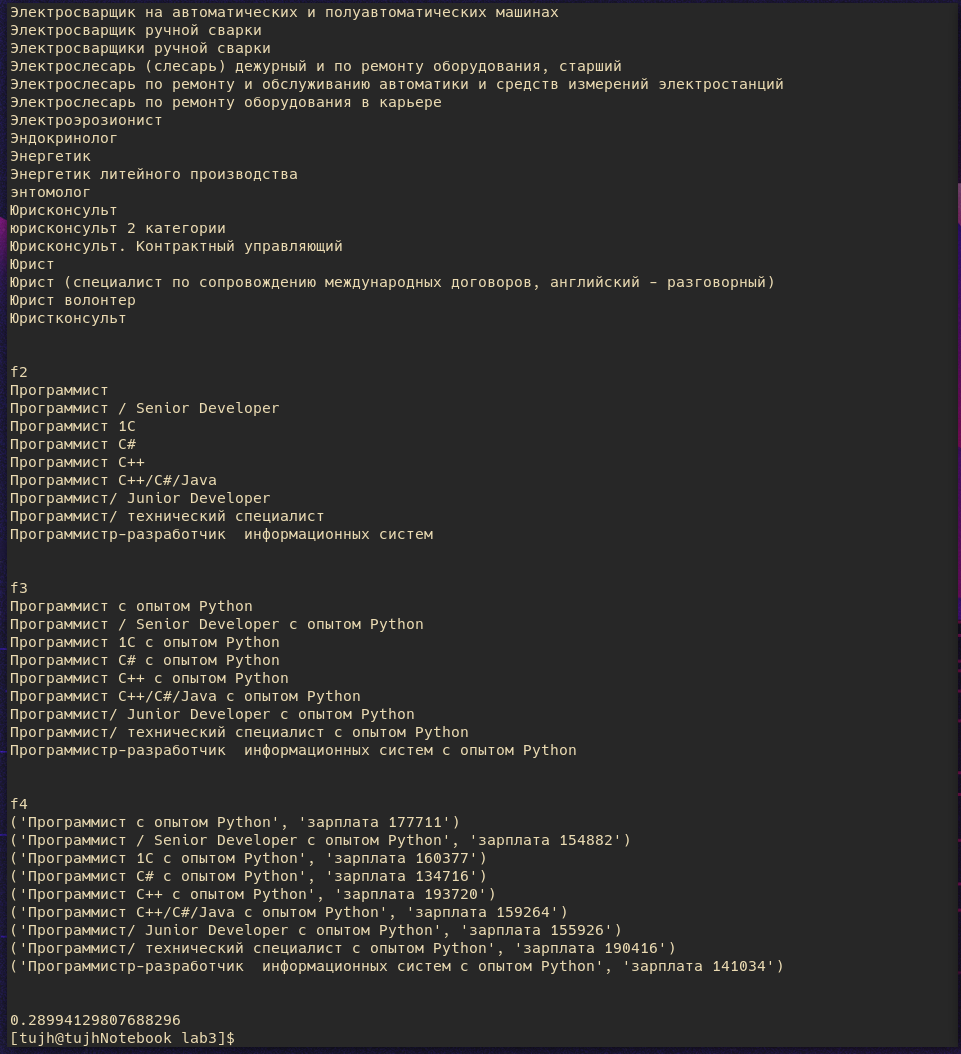
\includegraphics[width=\textwidth]{1.png}
		\end{figure}

\end{document}

